\documentclass[10pt]{article}
\usepackage[a4paper,margin=2.2cm]{geometry}
\usepackage[T1]{fontenc}
\usepackage{lmodern,microtype,booktabs,graphicx,amsmath,siunitx,xcolor,hyperref,url}
\sisetup{group-separator={,},group-minimum-digits=4}
\graphicspath{{figures/}}
\title{Supplementary material: system, platform measurements and farmer application}
\author{}\date{}
\begin{document}\maketitle
\noindent This supplement describes the production system that generated and serves the forecasts evaluated in the main paper. Every number is traceable through \texttt{docs/VERIFIED\_METRICS.md} in the repository.
\section{System design}\label{sec:system}

Figure~\ref{fig:arch} shows the data flow. Each component exists for a stated reason; the full rationale is in the
repository's \texttt{docs/ARCHITECTURE.md}.

\begin{figure}[t]
\centering
\small
\begin{verbatim}
 data.gov.in API --(key)--> adapter --+                      +-> bronze (raw JSON + offsets)
 AGMARKNET archive -------> replay ---+--> Kafka topic ------+-> silver (stream) --> alerts
                                           agri.prices.v1     |    shared standardize()
 raw CSV -> readers -> quality -> dedup -> silver (batch, Parquet, year=)
              -> harmonise -> sanity rule -> panel -> window features (<= t) -> targets (> t)
              -> baselines + MLlib (LR, Huber, RF, GBT-L2, GBT-L1) -> validation choice
              -> split conformal (validation) -> test once -> gold (Parquet)
              -> FastAPI + DuckDB (read-only) -> PWA (6 languages, offline)
\end{verbatim}
\caption{System data flow. Historical data takes the batch path; Kafka carries only incremental reports.}
\label{fig:arch}
\end{figure}

\paragraph{Batch layer.}
Scala jobs on Spark 4.2 DataFrames read the raw CSVs with explicit schemas, so no schema inference is needed.
They classify each record against seven quality rules and de-duplicate on a seven-column business key with grouped aggregation rather than a whole-row \texttt{distinct}, which had run out of memory in an earlier version.
The output is a year-partitioned Parquet silver layer.

\paragraph{Feature pipeline.}
Features are computed with window functions partitioned by entity and ordered by an integer day number:
\begin{itemize}
  \item 5 level, lag and return features;
  \item 10 rolling and range features over 7/30/90 calendar days, using \texttt{rangeBetween};
  \item 3 seasonal features at $t-365$ and the same-horizon change one year earlier;
  \item 4 same-day cross-sectional aggregates for the commodity, nationally and within the state;
  \item 3 calendar terms;
  \item the commodity index.
\end{itemize}
Every feature frame ends at offset~0 and every target frame starts at offset $+h\ge 1$.
A perturbation test multiplies all future prices, and all prices of another entity, by arbitrary factors.
It asserts that no feature at the origin changes, so any forward-looking or cross-entity window fails the test.
The job stages intermediate results as Parquet.
An earlier version persisted 33M-row frames with \texttt{DISK\_ONLY} caching and exhausted the development machine's disk.

\paragraph{Models.}
MLlib pipelines wrap each candidate: ridge regression and Huber regression on standardised features with one-hot commodity, and random forests and gradient-boosted trees on raw features with an indexed commodity.
The indexer and scaler are fitted on training rows only.
Fitted pipelines are persisted per experiment and applied unchanged when forecasts are published, so serving needs no separate model runtime.

\paragraph{Streaming layer.}
A Python adapter publishes canonical JSON events to a six-partition Kafka topic.
The adapter has retry with jittered exponential backoff, client-side rate limiting, atomic checkpoints and key redaction.
The message key is the business key, and the event id is a content hash.
Spark Structured Streaming writes two outputs:
\begin{itemize}
  \item a \emph{bronze} file sink with every record and its offsets;
  \item a \emph{silver} \texttt{foreachBatch} sink.
\end{itemize}
The silver path parses, quarantines unknown schema versions and malformed messages, and canonicalises with the same function as the batch layer.
It then drops exact re-sends by event id within a 10-day event-time watermark and scores alerts against batch-computed trailing statistics.
Writing each micro-batch to its own \texttt{batch\_id} directory makes replays idempotent.
The claimed guarantee is effectively-once output per offset range; end-to-end exactly-once from the government source is \emph{not} claimed.
Rolling features and forecasts are recomputed only by the batch layer. This trade-off keeps a single feature implementation.

\paragraph{Storage.}
A three-DataNode HDFS cluster (replication~3, 128\,MB blocks) holds the same layers under \texttt{/agri/\{raw, bronze, silver, features, models, predictions, gold, checkpoints, metadata\}}.
Directories are partitioned only by low-cardinality columns (year, horizon) to avoid creating tens of thousands of small files.
There is a single NameNode, so the store is not highly available.

\section{Streaming, storage and scalability measurements}
\subsection{Streaming}
We replayed \num{20000} real archived reports through a six-partition Kafka topic at 2,000 events/s with labelled faults: 5\% duplicates, 2\% late re-sends, 1\% malformed messages, and local reordering.
Of \num{21524} messages:
\begin{itemize}
  \item \num{20000} distinct events reached silver, with none missing and none never sent;
  \item \num{1317} duplicate or late copies were removed by watermarked de-duplication;
  \item 207 malformed messages were quarantined;
  \item none were dropped by the watermark.
\end{itemize}
The canonicalised streaming rows matched the batch canonicalisation of the same records in all 14 compared columns, with 0 mismatches.
The median per-batch producer-to-sink latency was 1.7\,s with a 2\,s trigger.
The red-team review found that an earlier version let a malformed message advance the event-time watermark and silently discard every later event. Unusable messages are now quarantined before the watermark, and a regression test covers this case.

\subsection{Storage and distributed execution}
The silver layer (692\,MB, \num{1743} files) was loaded into a three-DataNode HDFS with replication 3.
fsck reported no missing or corrupt blocks, and a file remained readable, with an identical checksum, while a DataNode was stopped.
All DataNodes share one physical disk, and there is a single NameNode.
On a containerised standalone Spark cluster (2 workers, 6 cores, 1\,GB executors) reading from HDFS, the aggregation workload processed 11.3M real rows in 9.2\,s and the window-feature workload in 14.4\,s.
These runs exercise the distributed code path (separate driver and executor JVMs, network shuffle, HDFS reads) but not multi-machine scaling.

\subsection{Single-host scalability}
\begin{figure}[t]
\centering
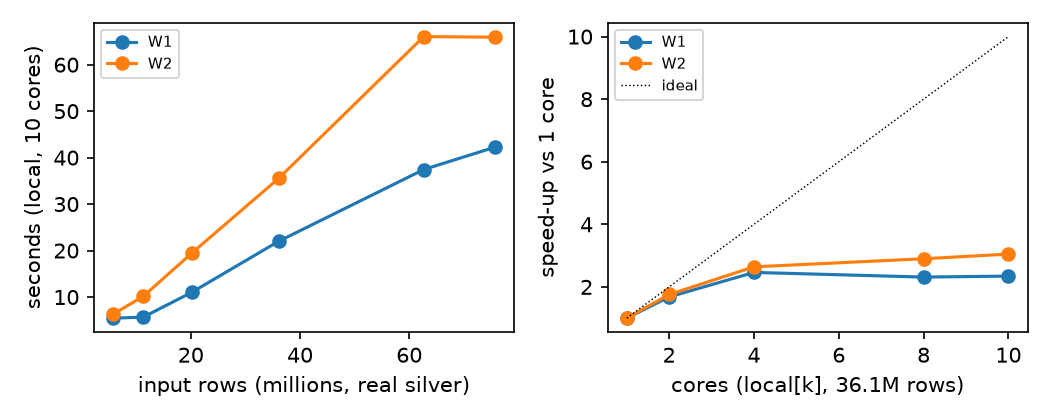
\includegraphics[width=0.9\linewidth]{scalability.png}
\caption{Left: run time against input size on the full silver layer (local mode, 10 cores). Right: speed-up against core count for 36.1M rows. W1 is an aggregation; W2 is per-entity window features.}\label{fig:scale}
\end{figure}
On one Apple M5 laptop (4 performance and 6 efficiency cores, 16\,GB), run time grows roughly linearly with input up to the full \num{75.6}M-row silver layer (Figure~\ref{fig:scale}).
Throughput is 1.6--2.0M rows/s for the aggregation and about 1.0M rows/s for the window features, with about 1\,GB of shuffle at full size and no disk spill.
Speed-up with cores flattens after four, matching the performance-core count: 2.5$\times$ for the aggregation and 3.0$\times$ for the window features at 10 cores.
The complete feature build for the forecasting panel (33M reports, 25 features, four targets) takes 8.3 minutes (\texttt{logs/f1\_build\_features.log}), and the full benchmark (38 model fits on 2M rows each, i.e.\ 32 candidates and 6 ablations, plus scoring of 6.4M test forecasts) takes 1\,h\,41\,min.

\section{Farmer application and decision support}\label{sec:app}

\paragraph{Design constraints.}
The intended users have entry-level Android phones (about 4\,GB of RAM), limited data plans and varied literacy.
The application is a progressive web app written in plain JavaScript modules, with no framework, CDN or build step:
\begin{itemize}
  \item 69\,KB of JavaScript in total, of which about 29\,KB loads for the first screen; the chart and the other screens are loaded lazily;
  \item a service worker precaches the application shell and fetches API data network-first with a timeout;
  \item when offline, it falls back to cached responses and labels them with the time they were saved.
\end{itemize}
All 264 interface strings, including decision reasons, warnings, errors, accessibility labels and a ten-topic farmer guide, exist in English, Tamil, Telugu, Malayalam, Hindi and Kannada.
Automated tests enforce identical key sets, identical placeholders and native-script content in every language.
Commodity names are always shown in their original published form, with a localised label from a reviewed dictionary where one exists.
The translations are AI-drafted and \emph{provisional} until reviewed by native speakers with agricultural vocabulary.

\paragraph{Freshness and provenance.}
Every price shows its report date and age.
A banner appears whenever the dataset is more than three days old.
During development the deployment served an archive ending on 2026-04-21, and labelled it a historical snapshot. After the official back-fill it serves data to 2026-10-22, labelled as official daily reports. It never calls batch-refreshed data ``live''.
Forecast screens show the model version, the source and licence, the measured test error for that commodity and horizon, and the measured coverage of the interval.

\paragraph{Decision cards.}
The cards turn the 80\% interval $[\ell_h,u_h]$ (on the log-return scale) into a transparent rule.
The holding cost is $c_h = c_0 + w\cdot h/7$: a fixed 1\% plus 5\% per week for perishables, or 1\% per week for durables.
These costs are placeholders that the farmer can edit.
\begin{itemize}
  \item \textsc{hold} if $\ell_h\ge\ln(1+c_h)$;
  \item \textsc{sell} if $u_h\le 0$;
  \item \textsc{compare} if a market in the same district reported a price at least 5\% higher within three days;
  \item \textsc{watch} otherwise.
\end{itemize}
Every card is labelled a \emph{market outlook}, not a profit recommendation, and has a ``Why am I seeing this?'' panel listing the interval, costs, accuracy and freshness.
The client recomputes the card when the farmer enters transport or holding costs.
Its test-period hit rates are reported in the main paper (Section 9).


\end{document}
